\begin{figure}[tbp]
\centering
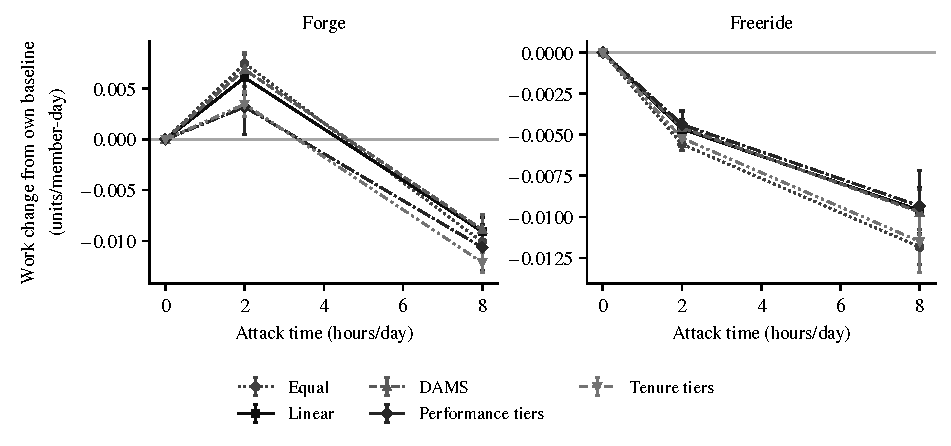
\includegraphics[width=\textwidth]{figures/results/attack-cost-effects.pdf}
\caption{Equal-time attack contrasts against each policy's own unattacked world. Eight independent worlds per cell, central record, 120 members, 60 days; fixed attacker cohort and ten active days. Points are sampled budgets, connected only as guides; bars are descriptive 95\% Monte Carlo intervals. Zero is the exact no-attack contrast, not an unexecuted missing cell. Forging raises observed claims and consumes time; free-riding also reduces real effort and help. These curves do not rank general security.}
\label{fig:attack-cost-effects}
\end{figure}
\begin{table}[tbp]
\centering\small
\caption{DAMS threat diagnostics under equal active-day time budgets.}
\label{tab:threat-diagnostics}
\begin{tabular}{lrrrrrr}
\toprule
Attack & \shortstack{Fraud\\committed} & \shortstack{Fraud initial\\rejections} & \shortstack{Honest review\\rejections} & \shortstack{Duplicate\\rejected} & Censored & \shortstack{Pending\\claims/appeals} \\
\midrule
None & 0.0 & 0.0 & 1449.2 & 0.0 & 0.0 & 914/4.6 \\
Forge & 229.5 & 401.0 & 1365.5 & 0.0 & 0.0 & 918/5.1 \\
Duplicate & 0.0 & 0.0 & 1666.0 & 405.8 & 0.0 & 1515/4.9 \\
Freeride & 0.0 & 0.0 & 1540.2 & 0.0 & 0.0 & 915/4.6 \\
Censor & 0.0 & 0.0 & 1585.2 & 0.0 & 43.9 & 872/5.1 \\
\bottomrule
\end{tabular}
\par\smallskip\begin{minipage}{0.96\textwidth}\footnotesize Eight matched independent worlds, central record, 120 members, 60 days, ten attack days at eight hour-equivalents/day. Entries are mean record counts; zero means no corresponding event, not missing data. Initial fraud rejections can later be appealed and committed; columns are nonexclusive events, not complementary detection rates. Honest review rejections count review events and can include duplicate submissions. Horizon stocks remain separate. Other policies and lower budgets are retained in the raw repository output.\end{minipage}
\end{table}
\begin{table}[tbp]
\centering\small
\caption{Equal-exposure and availability countercases for the same DAMS policy.}
\label{tab:record-countercases}
\begin{tabular}{lrrrr}
\toprule
Record & Equal exposure & Default exposure & Outage pending & Outage mean days \\
\midrule
Central & 41.9 & 41.9 & 912 & 4.91 \\
Witness & 41.9 & 21.2 & 2144 & 10.49 \\
Consensus & 41.9 & 0.0 & 3121 & 17.15 \\
\bottomrule
\end{tabular}
\par\smallskip\begin{minipage}{0.96\textwidth}\footnotesize Eight independent worlds per setting. The two censorship columns count censored records: equal exposure sets every substrate to 1; default sets central/witness/consensus to 1/.5/0. These are imposed assumptions. The outage lasts days 20--34 and only the stylized consensus commit path requires its quorum; central/witness worlds with the same dates are controls. Pending stock is measured at day 60; completed-only delay is in days. No actual distributed-client benchmark is represented.\end{minipage}
\end{table}
\begin{figure}[tbp]
\centering
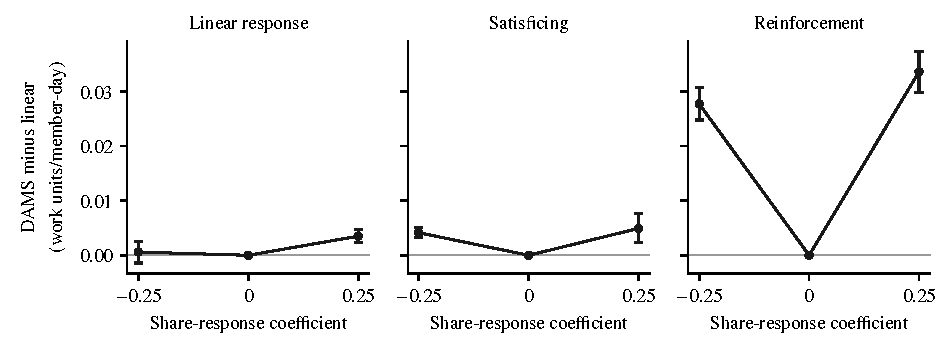
\includegraphics[width=\textwidth]{figures/results/response-boundaries.pdf}
\caption{Structural dependence of the DAMS--linear work contrast. Eight paired worlds per point; three effort rules and three predeclared response coefficients. Bars are descriptive 95\% Monte Carlo intervals conditional on each rule. Lines join sampled points without fitting. The zero channel is a mechanism null; negative responses provide an adverse case. Coefficients are unestimated design assumptions, not psychological measurements.}
\label{fig:response-boundaries}
\end{figure}
\begin{figure}[tbp]
\centering
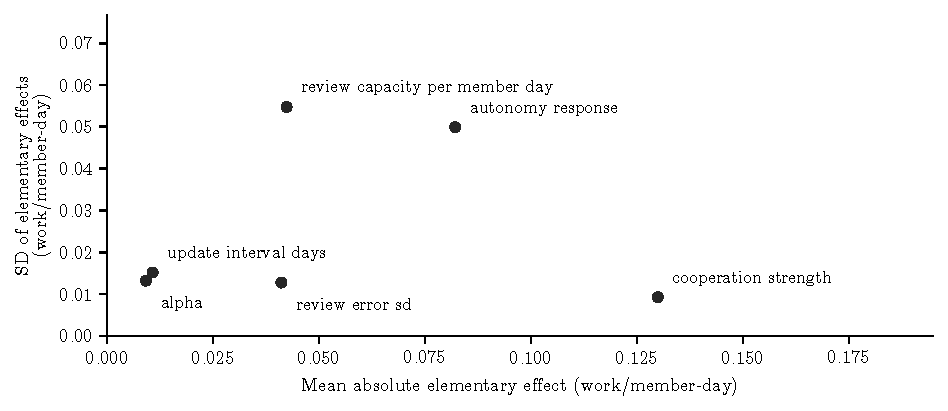
\includegraphics[width=\textwidth]{figures/results/sensitivity-screen.pdf}
\caption{Finite-difference screen over six independent design factors: eight randomized paths, three paired worlds at each step, four levels per factor. Horizontal position is mean absolute full-range elementary effect; vertical position is its path dispersion. This is a structural screening diagnostic, not Sobol indices or a probabilistic population variance decomposition. Input ranges and every path are retained in the repository.}
\label{fig:sensitivity-screen}
\end{figure}
\begin{table}[tbp]
\centering\small
\caption{DAMS--linear work contrasts across mechanistic stress contexts.}
\label{tab:context-results}
\begin{tabular}{lr}
\toprule
Synthetic context & Work difference [MC interval] \\
\midrule
noisy knowledge & 0.0034 [0.0028, 0.0041] \\
interdependent delivery & 0.0030 [0.0021, 0.0039] \\
distributed disruption & 0.0058 [0.0048, 0.0069] \\
high observation error & 0.0032 [0.0025, 0.0040] \\
cross principal confirmation & 0.0078 [0.0069, 0.0087] \\
review scarcity & 0.0100 [0.0091, 0.0110] \\
delayed accountability & 0.0023 [0.0016, 0.0031] \\
zero response & 0.0000 [0.0000, 0.0000] \\
reversed response & 0.0083 [0.0066, 0.0100] \\
\bottomrule
\end{tabular}
\par\smallskip\begin{minipage}{0.96\textwidth}\footnotesize Eight paired worlds per context, 120 members and 60 days. Intervals are descriptive 95\% normal Monte Carlo intervals; they do not include parameter or model uncertainty. Contexts change information, interdependence, site shocks, observation error, review resources, record assumptions, cadence or response. They are not calibrated industry, legal, demographic or sustainability cases.\end{minipage}
\end{table}
